% id: 0130
% book: RPM 중3-2 수학 · 01 삼각비
% section: 중단원 마무리하기
% figure: crop:fig-0130.png
% answer: ③
% answer_source: 답지
% variant_level: 0 (원본 전사)
% 이 파일은 build.mjs 가 items.json 에서 만든다. 고칠 때는 items.json 을 고친다.
\dmkichul{RPM 중3-2 수학 0130번 · 22쪽}
\noindent\begin{minipage}[t]{0.58\linewidth}\vspace{0pt}\raggedright 오른쪽 그림과 같이 $\angle\pt{A}=90^\circ$인 직각삼각형~$\pt{ABC}$에서 $\seg{DE}\perp\seg{BC}$이고 $\seg{AC}=2$, $\seg{BC}=3$일 때, $\cos x\times\tan y$의 값은?\end{minipage}\hfill\begin{minipage}[t]{0.4\linewidth}\vspace{0pt}\centering 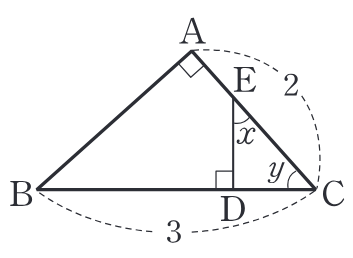
\includegraphics[width=84.6pt]{figures/fig-0130.png}\end{minipage}\par
\begin{choices32}{\rule[-3ex]{0pt}{8ex}$\dfrac{\sqrt{3}}{6}$}{\rule[-3ex]{0pt}{8ex}$\dfrac{\sqrt{5}}{6}$}{\rule[-3ex]{0pt}{8ex}$\dfrac{5}{6}$}{\rule[-3ex]{0pt}{8ex}$\dfrac{\sqrt{2}}{3}$}{\rule[-3ex]{0pt}{8ex}$\dfrac{\sqrt{3}}{3}$}\end{choices32}
